\documentclass[MSc,12pt]{wsuthesis}

%\usepackage[hdvipdfm]{graphics}
\usepackage{appendix}
\usepackage{color}
\usepackage{graphicx}
\usepackage{listings}
\usepackage{lscape}
\usepackage{pstricks}
\usepackage{setspace}
\usepackage{subfigure}
\usepackage{url}
\usepackage{verbatim}

% import figures
%\input{figures/figures.tex}

\begin{document}

\title{Anticipating Ray Tracing on Exascale Computers}

\author{Ellen Porter}

\submitdate{Your Submission Date}

\centerhdrstrue
\strhdrstrue

\dept{School of Electrical Engineering and Computer Science}

\chair{Robert R. Lewis}

\acknowledgment{
  Acknowledge whomever you want to here. (optional)
}

\abstract{
  Exascale computers, defined as being capable of performing at least
  one exaflop ($10^{18}$ floating point operations per second) are
  anticipated to emerge in the next several years. Reaching this scale
  of computation will require hardware and software changes for
  high-performance computing (HPC). Applications will need to adapt as
  the architecture of supercomputers change. Some studies suggest
  ``communication avoiding'' algorithms might be the most performant
  design for future systems. This has created an interest in the
  development of scalable visualization algorithms and techniques.

  In this paper we explore the impact exascale hardware will have on
  programming models and application design. We then look at one
  specific model, Concurrent Collections (CnC), and explore how we can
  use it and Intel's Embree Ray Tracing Engine to build a scalable ray
  tracing system with an emphasis on communication avoidance and
  extension for exascale. As exascale hardware does not yet exist,
  this work is speculative, but we hope it serves as a foundation for
  future discussion and work. %
}

\dedication{
  This is dedicated to ... (optional)
}

\preface

\chapter{Introduction}

% "\firstsection{Introduction}" is in "main.tex"

Exascale computers, by definition capable of performing at least one
exaflop ($10^{18}$ floating point operations per second), are
anticipated by 2018~\cite{kogge2013exascale}.
This will be several orders of magnitude greater than the fastest computers
currently available. Expectations will be high that software running on these computers will scale similarly.
Experience has shown, however, that such improvements will not be
achievable without similarly dramatic innovations in software,
particularly programming models and runtime design.

Until recent years, application performance has increased in
correspondence with Moore's law (which is not so much a law as an
observation): the number of transistors within an integrated circuit
doubled approximately every two years. As we reached a limit on the
number of transistors a single core could contain, hardware architects
had to look for other ways to keep up with performance advancement
expectations. The most common solution today is multiple cores per
chip. In order to take advantage of these hardware advances,
applications often require redesign.

In addition to the changing software architectures, the amount of
output data expected from high-performance computing (HPC)
applications also scales with compute power: larger computers are
expected to manage larger amounts of data. An additional expectation
is that of ``real time'', dynamic display of data.

These demands have produced a need for rendering and visualization
systems which can take advantage of distributed systems. These systems
may be stand-alone or they may add functionality to existing HPC
applications. This paper proposes one such system for ray tracing, a
commonly-used rendering technique, using the Intel Concurrent
Collections (CnC) programming model. Although CnC runs on current
distrbuted hardware, it is ultimately intended for use on exascale
computers.


%%% Local Variables: 
%%% mode: latex
%%% TeX-master: "main"
%%% End: 


\chapter{Background}

\section{Reaching Exascale}
\label{sec:reaching}

Until 2004, performance of single-core microprocessors increased as
predicted as a result of smaller and faster transistors being
developed (i.e. Moore's Law). At that time, this trend shifted as we
reached an inflection point caused by a chip’s power dissipation
~\cite{kogge2013exascale}. Unable to sufficiently and inexpensively
cool a chip, chip designers looked for other ways to increase
performance. This came in the form of multi-core processors, which are
now the building blocks of many HPC (and other) systems.

The introduction of multi-core processors on each node of a cluster
caused a shift in parallel application design. Programs using the
cross-platform standard Message Passing Interface (MPI) library
~\cite{Snir:1998:MCR:552013} could not efficiently exploit parallelism
on individual nodes without a rewrite of the underlying algorithms.
The Open Multi-Processing (OpenMP) ~\cite{openmp08} library presented
a cross-platform standard for parallel programming on multicore nodes,
which led to the emergence of hybrid systems that mixed MPI and
OpenMP. The cluster would run a collection of MPI processes, one per
node, and each node would then execute an OpenMP program redesigned
from the original single-threaded program which used a fixed number of
threads to execute a single work-sharing construct, such as a parallel
loop ~\cite{gropp2013programming}.

Although the exact form of an exascale ecosystem is unknown, research
suggests that data movement will overtake computation as the dominant
cost in the system.
% RRL: It would be nice to cite something here.
This results from the primary means to increase parallelism is
expected to be on-chip, with some predictions
% RRL: citation?
suggesting hundreds or even thousands of cores
per chip die.
As a result, we will would see a higher available bandwidth on
chip along with lower latencies for communication within a node.
% RRL: It is not logical that lower latency should lead to a need to
%   reduce commmunication, *unless* we're talking about off-chip
%   communication.
The
lower overhead within a chip provides a significant incentive to
develop ``communication avoiding'' algorithms.

Two means to avoid communication are, first, to re-compute values
instead of communicating results when possible and, second, to take
account of the need to minimize communication when partitioning the
algorithm into parallel functional units.

Many of our current programming models lack the semantics necessary to
implement communication-avoiding algorithms. As a result, new
languages with additional semantics are being proposed for exascale
systems. A common theme among these languages is the ability to
statically declare data dependencies and data locality information.
These additional details can then be used by the runtime to aid in
scheduling and anticipatory data movement.

\subsection{Task-Based Programming Models}

One class of programming model that may map well onto exascale systems
are task-based models. They tend to be declarative: An application is
broken down into chunks of work and the inputs and outputs to that
work are declared in the language semantics. Their explicit data
dependencies allow the runtime to optimally schedule and execute the
tasks, or chunks of work, in the application.

Execution can often be further improved by the implementation of a
secondary specification (a file, typically) separate from the program
that provides ``hints'' to the runtime. The key difference between many
task-based models and more traditional programming models is the
movement from compute-centric to data-centric application design.
Algorithms are designed around the data a task needs to execute and
the data it will produce rather than designed around the computation.

%%% Local Variables: 
%%% mode: latex
%%% TeX-master: "main"
%%% End: 



\section{Limitations of Current Ray Tracing Algorithms}

% RRL: I will add "lmprop" of ray tracer here.

Traditional ray tracing algorithms are embarrassingly parallel as no
primary ray depends on any other ray. The data needed by each
individual ray, however, varies widely as its path is traced,
especially as regards secondary or other rays. Acceleration
structures, such as k-d trees have been developed to increase ray
tracing performance. As the data scales up however, it is no longer
possible to store an entire data set in an acceleration structure in
shared memory.

One solution is to implement data decomposition. Each node on a
distributed system is then responsible for a subset of the domain.
Primary rays and secondary rays are then communicated across nodes as
the algorithm executes. These types of models typically rely on
expensive preprocessing steps that help to balance both the data
distribution and rendering work evenly across nodes
~\cite{navratil2014dynamic}.

%%% Local Variables: 
%%% mode: latex
%%% TeX-master: "main"
%%% End: 


\chapter{Previous Work}

Cite previous work (using bibtex).

\chapter{Design}

\section{The CnC Programming Model}
\label{sec:cnc}

The Concurrent Collections Programming Model (CnC), developed by
Intel, is one such data-centric programming model. Its deterministic
% RRL: "task-based" vs. "data-centric" -- choose one
semantics allow a task-based runtime to programmatically exploit
parallelism. In addition, it allows for a secondary file, called a
tuning spec, to provide additional hints to improve performance.

\begin{figure}[t!]
  \centering
  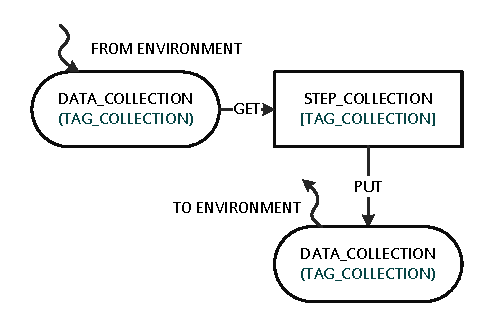
\includegraphics[width=0.5\textwidth]{drawings/CnCExample.pdf}
  \caption{CnC Graph Semantics}
  \label{fig:cnc_graph}
\end{figure}

The CnC model can be thought of as a producer-consumer paradigm where
data is produced and consumed by tasks, or ``steps'' in CnC
terminology. The produced and consumed data is declared explicitly in
an input file, known as a ``graph file''. The steps themselves are
also entities that can be produced. When a step produces another step,
this is known as a ``control dependency'' and is also declared in the
graph file.

Figure~\ref{fig:cnc_graph} shows a graph file. The rectanglees are
``step collections'', the ``data collections'' are ovals, and the
dependencies are directed edges between them. The title of a step
collection is usually a descriptive verb and the title of a data
collection is usually a descriptive noun. The control dependencies are
not shown. A text description of Figure~\ref{fig:cnc_graph} (which
includes control information) is provided to CnC when designing a CnC
application.
% RRL: "designing", not "running"?
Section~\ref{sec:raytracing} shows an example of this.

By declaring all dependencies between steps and data, the specifics
regarding how the algorithm is executed is abstracted out of the
implementation. For example: It is clear what data is needed by a
given step, so if that data has not been produced yet, the step will
not be scheduled. This allows the runtime to optimally decide when and
where to schedule computation. By way of contrast, in a conventional
multithreaded program, it is the responsibility of the programmer to
guarantee that a thread's inputs are available and consequently start
the thread.

For some more complicated semantics, additional hints can be provided
to the runtime through a ``tuning specification''. As the tuning
specification usually is in a separate file, this makes it easy to run
the same program on different architectures, as no rewrites of the
application are necessary to switch platforms: just the tuning
specification.

\subsection{Language Specifics}
The CnC model is built on three key constructs; step collections, data
collections, and control collections ~\cite{budimlicconcurrent}. A
step collection defines computation, an instance of which consumes and
produces data. The consumed and produced data items belong to data
collections. Data items within a data collection are indexed using
item ``tags'': tuples that, like primary keys, can uniquely identify a
data item in the data collection. Finally, the control collection
describes the prescription, or creation, of step instances. The
relationship between these collections as well as the collections
themselves are defined in the graph file.

Developing a CnC application then begins with designing the graph
file. An algorithm is broken down into computation steps, instances of
which correspond to different input arguments. These steps, along with
the data collections become nodes, in the graph. Each step can
optionally consume data, produce data, and/or prescribe additional
computation. These relationships: producer, consumer, and control,
define the edges of the graph and will dynamically be satisfied as the
program executes.

The next and final required step in producing a CnC application is to
implement the step logic. The flow within a single step is: consume,
compute, and produce. This ordering is required as there is no
guarantee the data a step needs will be ready when the step begins
executing. This is due to steps being preemptively scheduled when they
are prescribed. Most of the time the data \emph{will} be ready when a
step begins execution, but occasionally and often due to an
implementation error, a step’s data may never be available.
Internally, if the data is not ready when a step begins execution
it will halt execution and try again later. To improve performance,
hints can be provided through the tuning specification to increase the
likelihood that steps are schedule for execution when their required
input data is ready.

\subsection{Example}

\begin{figure}[!tb]
  \centering
  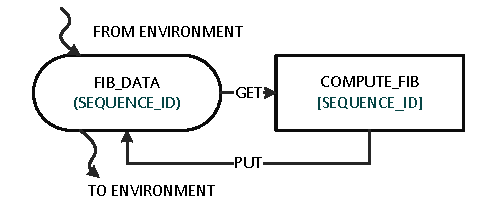
\includegraphics[width=0.5\textwidth]{drawings/FibExample.pdf}
  \caption{A CnC Graph to Compute the Fibonacci Sequence}
  \label{fig:fib_graph}
\end{figure}

% apparently putting this here makes it show up on the top of page 3, where I want it
\begin{figure*}[t]
  \centering
  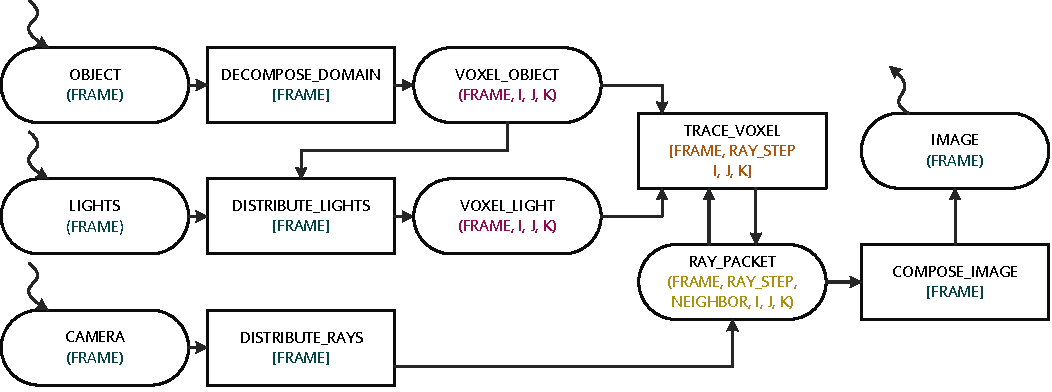
\includegraphics[width=\textwidth]{drawings/CnC.pdf}
  \caption{CnC Graph}
  \label{fig:cnc}
\end{figure*}

Figure~\ref{fig:fib_graph} shows an example of a
simple iterative implementation of the Fibonacci sequence. This
application consists of one step, COMPUTE\_FIB, which takes the
previous two computed values as input and produces the next value in
the sequence. One data collection, FIB\_DATA, exists for the
application. Data within the collection is indexed by a tag consisting
of the sequence number. Tags 1-5, then index the values 1,
1, 2, 3, 5, respectively. The first two values of the data collection
are produced by the environment, the rest of the values in the
collection are produced as needed by COMPUTE\_FIB. A tag exists for
COMPUTE\_FIB as well. We can index this collection by the integer
sequence a particular instance will produce. For example, the step
% RRL: What do you mean by "integer sequence"? The *whole* Fibo sequence?
instance at tag 3 will consume the data at tag 1 and 2, and produce
data at tag 3. Specifically it will consume 1, 1 and produce 2.
The number of steps executed in this example is provided by the 
environment.

%%% Local Variables: 
%%% mode: latex
%%% TeX-master: "main"
%%% End: 



\chapter{Implementation}

\section{Ray Tracing for Exascale}

When designing our ray tracer for exascale we focused on two key aspects, producing a task based application with an emphasis on avoiding communication.  For simplicity we consider only ray tracing scenes without reflection or refraction, although our proposed algorithm can be extended to handle either in the future.  Our algorithm uses a simple voxel decomposition to split the work required to trace a scene.  Primary camera rays are then sent into the system and propagating through the domain. As secondary rays introduce most of the uncertainty in the amount of communication necessary in a ray tracing algorithm, we introduce a pre-processing technique that distributes light information to each voxel prior to tracing the scene.  This allows the ray tracing step within each voxel to be completely independent of the data in the rest of the domain.  Using this algorithm we can predict an upper bound on the amount of communication necessary (a scene that contains no data), and extrapolate from there rough estimates on how our algorithm might perform on an exascale system.

\subsection{Implementation}

We chose to implement our ray tracer using Intel’s implementation of CnC which is built on top of their Thread Building Blocks (TBB) library as it has the potential to run on today’s systems as well as next generation exascale architecture.  Figure \ref{fig:cnc} shows the proposed CnC graph for our distributed ray tracer. Data collections, step collections and the dependencies between them are represented in the graph. The tags corresponding to each collection are also shown within the graph node. The control collection for the proposed model is static for all steps and defined in an initialization step. The graph begins execution when the object, lights, and camera data are provided, and terminates when it produces an image.

\subsection{Tags}

The tags are different for many of the data and step collections but share common elements.  FRAME refers to one specific frame in the case of an animation.  INSTANCE refers to the current iteration. I, J, K are iterators over spatial data.

\subsection{Data Collections}

OBJECT contains input data for the scene from the environment.  It is in the form of .obj.  DECOMPOSE\_DOMAIN splits this data into voxels and produces VOXEL\_OBJECT, object data for a given voxel.  Triangles that span multiple voxels are duplicated.  The LIGHTS data collection contains data pertaining to any light sources.  VOXEL\_LIGHT contains the same information as LIGHTS plus a traced light mesh for each wall of a voxel.  CAMERA contains the location and direction of the camera.  RAY\_PACKET contains all the rays that intersect a voxel wall for a given wall and iteration.  IMAGE contains the final image data.

\subsection{Step Collections}

\subsubsection{Decompose Domain}

DECOMPOSE\_DOMAIN takes the data to be traced as input and produces subsets of that data based on voxel decomposition.  As load balancing is not a concern a fast uniformly spaced geometric distribution is sufficient.  The number of voxels produced is set at runtime and should be more than the number of nodes available.

\subsubsection{Distribute Lights}

In order to reduce communication of secondary rays, DISTRIBUTE\_LIGHTS lights is responsible for distributing light information to each voxel.  This guarantees each voxel will only need to communicate with its direct neighbors.  The light information produced for each voxel contains the original light sources as well as a light source mesh for each light and each wall of the voxel.  The mesh is produced by tracing rays from each light source to uniformly spaced points along a voxel wall, see Figure \ref{fig:light}.  Where the rays intersect the wall, new point or directional light sources are created.  If the ray is blocked, the node in the light mesh is tagged as in shadow.

\begin{figure}[!htb]
\centering
\begin{subfigure}{.49\columnwidth}
 \centering
  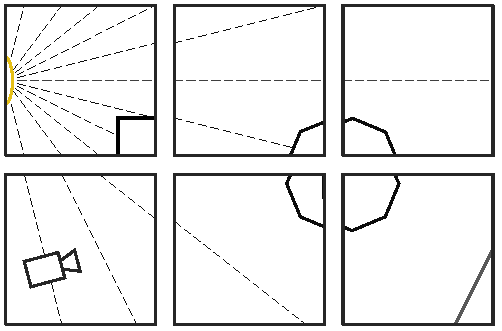
\includegraphics[width=.98\columnwidth]{drawings/Lights1.pdf}
  \caption{Initial light rays}
\end{subfigure}
\begin{subfigure}{.49\columnwidth}
 \centering
  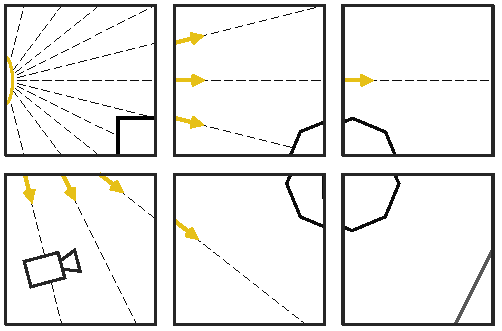
\includegraphics[width=.98\columnwidth]{drawings/Lights2.pdf}
  \caption{Point light sources}
\end{subfigure}
\caption{Light Ray Distribution}
\label{fig:light}
\end{figure}

\subsubsection{Distribute Rays}

DISTRIBUTE\_RAYS is responsible for sending each voxel its first iteration of ray information.  This is an empty set of data for all voxels except the voxel containing the camera if the camera is positioned within the domain.  If the camera is outside the domain, multiple voxels may receive data.

\subsubsection{Trace Voxel}

TRACE\_VOXEL is the heart of the application. This step executes multiple times for each voxel, depending on the size of the domain.  Each time TRACE\_VOXEL executes, it consumes ray packets from each of its neighbors. It then traces the rays over its subset of the domain. If a ray intersects with an object, secondary rays from each light source are considered if the corresponding point or directional light source from the voxels light mesh is not in shadow. Rays that do not intersect objects within the voxels and reach the voxels walls are collected and passed to the corresponding neighbor on the next iteration. See figure \ref{fig:trace}.  Because we are not considering reflection or refraction, we know the maximum amount of times we will have to communicate a single ray across voxel borders in the worst case is proportional to domain size.  This allows us to prescribe the correct number of instances of TRACE\_VOXEL in an initialization step.  For the example in figure \ref{fig:trace} that maximum is 3.  As each CnC step instance will eventually be executed on a single node of a cluster we plan to integrating with Embree, Intel’s ray tracing kernel, in order to optimize per node performance.

\begin{figure}[!htb]
\centering
\begin{subfigure}{.49\columnwidth}
 \centering
  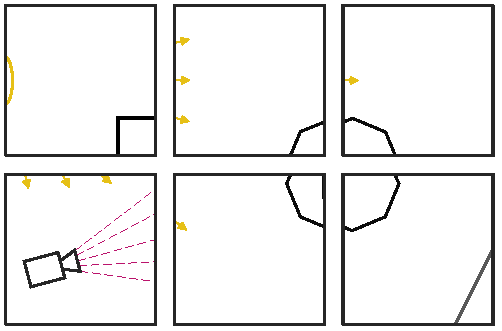
\includegraphics[width=.98\columnwidth]{drawings/Trace1.pdf}
  \caption{Distribute rays}
\end{subfigure}
\begin{subfigure}{.49\columnwidth}
 \centering
  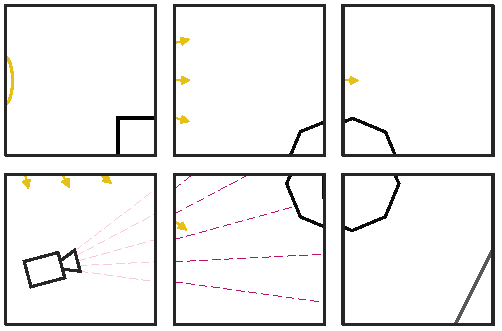
\includegraphics[width=.98\columnwidth]{drawings/Trace2.pdf}
  \caption{Trace voxel; ray step 1}
\end{subfigure}
\begin{subfigure}{.49\columnwidth}
 \centering
  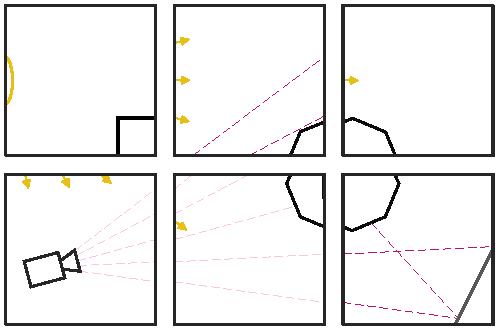
\includegraphics[width=.98\columnwidth]{drawings/Trace3.pdf}
  \caption{Trace voxel; ray step 2}
\end{subfigure}
\begin{subfigure}{.49\columnwidth}
 \centering
  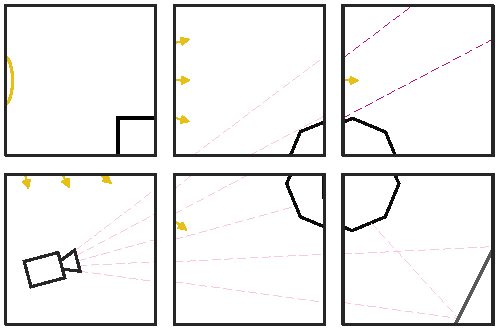
\includegraphics[width=.98\columnwidth]{drawings/Trace4.pdf}
  \caption{Trace voxel; ray step 3}
\end{subfigure}
\caption{Trace Voxel}
\label{fig:trace}
\end{figure}

\subsubsection{Produce Image}
When all step instances of TRACE\_VOXEL have completed, the final set of ray packets is produced.  Each ray in that packet contains the information necessary to produce the final image; merging these is the responsibility of the PRODUCE\_IMAGE step.  

\subsection{Textual CnC Graph File}
To give a more concrete example of how the CnC graph file is implemented, we are including a simplified version the textual representation of TRACE\_VOXEL.  In addition to the step declaration, the code includes the SCENE and RAY\_PACKET data collections as well as the control dependencies from the environment for TRACE\_VOXEL. \\

% Code..
\begin{lstlisting}[language=c,basicstyle=\tiny]
/******************************************************************************
//* Item collection declarations */

// scene data for each voxel, produced by decompose_domain
[ scene_data *scene : frame, i, j, k ];

// ray data passed to neighbors, produced by camera and trace_voxel
[ ray_packet *rays : frame, ray_step, neighbor, i, j, k ];

/******************************************************************************
//* CnC steps */

( trace_voxel : frame, ray_step, i, j, k )
<- [ scene: frame, i, j, k],
   [ rays : frame, ray_step  , 0, i  , j  , k   ] $when(i<#voxels_i-1),
   [ rays : frame, ray_step  , 1, i  , j  , k   ] $when(i>0),
   [ rays : frame, ray_step  , 2, i  , j  , k   ] $when(j<#voxels_j-1),
   [ rays : frame, ray_step  , 3, i  , j  , k   ] $when(j>0),
   [ rays : frame, ray_step  , 4, i  , j  , k   ] $when(k<#voxels_k-1),
   [ rays : frame, ray_step  , 5, i  , j  , k   ] $when(k>0)
-> [ rays : frame, ray_step+1, 0, i-1, j  , k   ] $when(i>0),
   [ rays : frame, ray_step+1, 1, i+1, j  , k   ] $when(i<#voxels_i-1),
   [ rays : frame, ray_step+1, 2, i  , j-1, k   ] $when(j>0),
   [ rays : frame, ray_step+1, 3, i  , j+1, k   ] $when(j<#voxels_j-1),
   [ rays : frame, ray_step+1, 4, i  , j  , k-1 ] $when(k>0),
   [ rays : frame, ray_step+1, 5, i  , j  , k+1 ] $when(k<#voxels_k-1);

/******************************************************************************
//* Input output relationships from environment */

( $initialize: () )
-> (trace_voxel : $range(0, #num_frames), $range(0, #ray_steps),
           $range(0, #voxels_i), $range(0, #voxels_j), $range(0, #voxels_k));


\end{lstlisting} 

Under the \emph{Item collection declaration} section we see two item collections being declared.  Once for the scene and one for the ray packets.  Instances of the scene are indexed using frame, i, j, and k which correspond to the frame in the case of an animation and the 3-dimensional identifier for a given voxel.  Ray packets are indexed similarly but also include an entry for the current ray step as well as a neighbor identifier.

Under \emph{CnC steps} we see the declaration for TRACE\_VOXEL.  Each instance of trace voxel is indexed using the frame, the voxels i, j, k and the current ray step.  The specific instances of the scene and rays data consumed and produced by TRACE\_VOXEL can be declared using the steps tag.  The step will always consume its scene data.  It will then optionally consume a ray packet for each of its voxel walls, assuming it is not on an edge.  For each wall not on an edge, an instance of the step will produce a packet of rays for 
each neighboring voxels shard wall.

Under \emph{Input output relationships from environment} we see the control for TRACE\_VOXEL.  In the initialize step we will produce an instance of TRACE\_VOXEL for every frame in our animation, for every step in our ray steps, and for each voxel in our domains decomposition.

%%% Local Variables: 
%%% mode: latex
%%% TeX-master: "main"
%%% End: 


\chapter{Evaluation}


%%% Local Variables: 
%%% mode: latex
%%% TeX-master: "main"
%%% End: 


\chapter{Conclusions}

\section{Conclusions and Future Directions}


\subsection{Future Directions}

\subsubsection{Hierarchy}

\subsubsection{Dynamic scenes}

\subsubsection{checkpoint and restart} 

\subsubsection{Global illumination}


%%% Local Variables: 
%%% mode: latex
%%% TeX-master: "main"
%%% End: 


\chapter{Future Work}

What sort of things could follow from this work?

\newpage
\singlespacing
\bibliographystyle{plain}
\bibliography{bibliography}

\appendix
% If you really *must* include source code.
% \chapter{Source Code}
% \begin{figure}[!htb]
  \begin{center}
    
\begin{algorithm}
/******************************************************************************
// * CnC Ray Tracer
// *
// * Author: Ellen Porter (ellen.porter@wsu.edu)
// *         Washington State University
// *
//****************************************************************************/

/******************************************************************************
// * Graph parameters */
$context {
  int voxels_i;   // decomposed domain size
  int voxels_j;
  int voxels_k;
  int num_frames; // frames to trace
};

/******************************************************************************
//* Item collection declarations */
//object data for each voxel, produced by decompose_domain
[ voxel_object *object_data : frame, i, j, k ];
// light data for each voxel, produced by distribute_lights
[ voxel_light *light_data : frame, i, j, k ];
// ray data passed to voxels, produced by distribute_rays
[ rays *primary_rays : frame ];
// ray data produced by trace_voxel
[ rays *traced_rays : frame, i, j, k ];

/******************************************************************************
//* CnC steps */
( decompose_domain : frame )
-> [ object_data : frame, 
     $range(0, #voxels_i), $range(0, #voxels_j), $range(0, #voxels_k) ];
( distribute_lights : frame )
<- [ object_data : frame, 
     $range(0, #voxels_i), $range(0, #voxels_j), $range(0, #voxels_k) ]
-> [ light_data : frame, 
    $range(0, #voxels_i), $range(0, #voxels_j), $range(0, #voxels_k) ];
( distribute_rays : frame )
-> [ primary_rays : frame ];
( trace_voxel : frame, i, j, k )
<- [ object_data  : frame, i, j, k],
   [ light_data   : frame, i, j, k],
   [ primary_rays : frame ]
-> [ traced_rays  : frame, i, j, k];
(compose_image : frame )
<- [ traced_rays : frame, 
     $range(0, #voxels_i), $range(0, #voxels_j), $range(0, #voxels_k)];

/******************************************************************************
//* Input output relationships from environment */
( $initialize: () )
-> (decompose_domain : $range(0, #num_frames)),
   (distribute_rays  : $range(0, #num_frames)),
   (trace_voxel      : $range(0, #num_frames), 
       $range(0, #voxels_i), $range(0, #voxels_j), $range(0, #voxels_k)),
   (compose_image    : $range(0, #num_frames));
( $finalize: () );

\end{algorithm} 
  \end{center}
  \caption{Textual CnC graph file}
  \label{fig:cnc-graph-text}
\end{figure}



\end{document}
